\documentclass[a4paper, 11pt]{article}
\usepackage{geometry}
\usepackage{indentfirst}
\usepackage{setspace}
\usepackage{amsmath}
\usepackage{graphicx}
\usepackage{wrapfig}
\usepackage{caption}
\usepackage{indentfirst}
\setlength{\parindent}{20pt}
\usepackage{amssymb}
\usepackage{float}

\graphicspath{ {./images/} }
\geometry{left=2.5cm, right=2.5cm, top=2.5cm, bottom=2.5cm}

\begin{document}	
	\title{Exercise \# 2. Iterative Methods For Linear Systems. }
	\author{{\small Alexandre Rodrigues (2039952)}}
	\date{\today}
	
	\maketitle
		\section*{Question 1}
		My implementation is slower to converge...
		
		
		
		
		\section*{Question 2}
		
		
		The spectral condition number of A is 
		\begin{equation}
			k = \frac{\lambda_{max}(A)}{\lambda_{min}(A)}
		\end{equation}
	
		\begin{table}[H]
			\centering
			\begin{tabular}{c|c|c|c|c|c|c|c}
				\textbf{nx} & \textbf{h} 			& \textbf{k} 			 & \textbf{sqrt(k)}	& \textbf{iters CG} & \textbf{iters IC(0)} & \textbf{iters $IC(10^{-2})$} & \textbf{iters $IC(10^{-3})$} \\ \hline
				$ 102 $ & $ 1.0000 \times 10^{-4} $ & $ 6.0107 \times 10^3 $ & $ 77.5288 $ 		& $ 283 $ & $ 87 $ & $ 45 $ & $ 17 $ \\ \hline
				$ 202 $ & $ 2.5000 \times 10^{-5} $ & $ 2.3810 \times 10^4 $ & $ 154.3039 $ 	& $ 532 $ & $ 159 $ & $ 78 $ & $ 30 $ \\ \hline
				$ 402 $ & $ 6.2500 \times 10^{-6} $ & $ 9.4770 \times 10^4 $ & $ 307.8473 $ 	& $ 948 $ & $ 282 $ & $ 137 $ & $ 53 $\\ \hline
				$ 802 $ & $ 1.5625 \times 10^{-6} $ & $ 3.7814 \times 10^5 $ & $ 614.9304 $ 	& $ 1792 $& $ 533 $ & $ 258 $ & $ 97 $ \\ \hline
			\end{tabular}
			\caption{all data}
			\label{table:ex2}
		\end{table}	
	
		\begin{table}[H]
			\centering
			\begin{tabular}{c|c|c|c|c|c}
				\textbf{nx} & \textbf{h} & \textbf{iters CG} & \textbf{iters IC(0)} & \textbf{iters $IC(10^{-2})$} & \textbf{iters $IC(10^{-3})$} \\ \hline
				$ 102 $ & $ 1.0000 \times 10^{-4} $ 	& $ 283 $ & $ 87 $ & $ 45 $ & $ 17 $ \\ \hline
				$ 202 $ & $ 2.5000 \times 10^{-5} $ 	& $ 532 $ & $ 159 $ & $ 78 $ & $ 30 $ \\ \hline
				$ 402 $ & $ 6.2500 \times 10^{-6} $  	& $ 948 $ & $ 282 $ & $ 137 $ & $ 53 $\\ \hline
				$ 802 $ & $ 1.5625 \times 10^{-6} $ 	& $ 1792 $& $ 533 $ & $ 258 $ & $ 97 $ \\ \hline
			\end{tabular}
			\caption{Iterations for each value of nx}
			\label{table:ex2-1}
		\end{table}	
		
		$ h = \frac{1}{N} = \frac{1}{(nx-2)^2} $
		
		
		
		\section*{Question 3}
		show theoretically ??
		only 1 iter??
		
		
		Matlab PCG without preconditioning, My PCG with L as identity matrix
		\textbf{\begin{figure}[H]
				\centering
				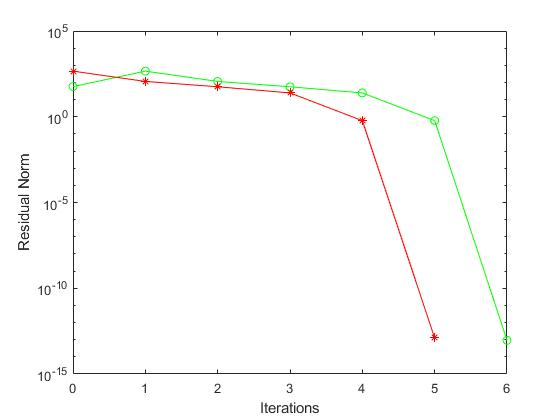
\includegraphics[width=.6\linewidth]{ex3_NoPrec.jpg}
				\caption{semilogy plot ex3 no preconditioning}
				\label{fig:ex3_NoPrec}
		\end{figure}}
	
		\begin{table}[H]
			\centering
			\begin{tabular}{c|c|c|c}
				\textbf{Method} &  \textbf{Iterations} 	& \textbf{Final Residual} 		& \textbf{Computational Time} 	\\ \hline
				Matlab PCG		& 			$6$ 		& $ 9.2128 \times 10^{-14} $ 	& $ 0.021 s $	\\ \hline	
				My PCG 			& 			$5$			& $ 1.2744 \times 10^{-13} $	& $	0.012 s $	\\ \hline
			\end{tabular}
			\caption{Iterations for each value of nx, no preconditioning}
			\label{table:ex3_NoPrec}
		\end{table}
		
		
		
		
		\section*{Question 4}		
		\begin{figure}[H]
			\centering
			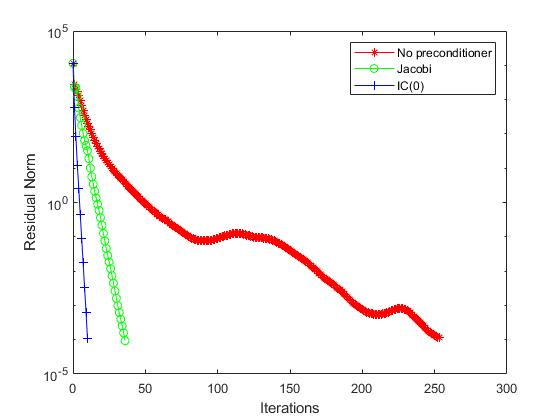
\includegraphics[width=.6\linewidth]{ex4.jpg}
			\caption{semilogy plot ex4}
			\label{fig:ex4}
		\end{figure}
		
		
		\section*{Question 5}
		
		
		\section*{Question 6}
		
			
		
		With L
		
		\begin{table}[H]
			\centering
			\begin{tabular}{c|c|c|c}
				\textbf{Method} &  \textbf{Iterations} 	& \textbf{Final Residual} 		& \textbf{Computational Time} 	\\ \hline
				GMRES 			& 			1 			& $ 3.8481 \times 10^{-16} $	& $ 0.027 s $	\\ \hline	
				My PCG 			& 			1			& $ 1.7554 \times 10^{-17} $	& $ 0.003 s $	\\ \hline
			\end{tabular}
			\caption{Iterations for each value of nx}
			\label{table:ex4_c_prec}
		\end{table}	
	
		GMRES without preconditioning, My PCG with L as identity matrix
			
		\begin{table}[H]
			\centering
			\begin{tabular}{c|c|c|c}
				\textbf{Method} &  \textbf{Iterations} 	& \textbf{Final Residual} 		& \textbf{Computational Time} 	\\ \hline
				GMRES			& 			$6$ 		& $ 3.0413 \times 10^{-14} $ 	& $ 0.102 s $	\\ \hline	
				My PCG 			& 			$5$			& $ 1.0468 \times 10^{-13} $	& $ 0.012 s $	\\ \hline
			\end{tabular}
			\caption{Iterations for each value of nx, no preconditioning}
			\label{table:ex4_c_NoPrec}
		\end{table}
	
		\begin{figure}[H]
			\centering
			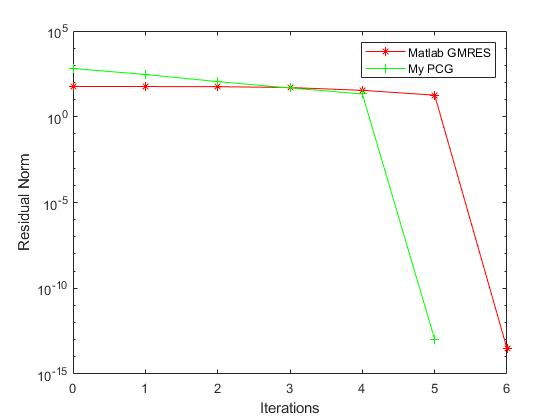
\includegraphics[width=.6\linewidth]{ex6.jpg}
			\caption{semilogy plot ex6, GMRES without preconditioning, My PCG with L as identity matrix}
			\label{fig:ex6_c_NoPrec}
		\end{figure}
		
		
		
		\section*{Question 7}
		
		\begin{table}[H]
			\centering
			\begin{tabular}{c|c|c|c}
				\textbf{Restart} &  \textbf{Iterations} 	& \textbf{Final Residual} 		& \textbf{Computational Time} 	\\ \hline
				10			& 			$1149$ 		& $ 9.6915 \times 10^{-13} $ 	& $ 2.235 s $	\\ \hline	
				20			& 			$739$		& $ 9.6140 \times 10^{-13} $	& $ 1.443 s $	\\ \hline
				30			& 			$88$ 		& $ 6.7203 \times 10^{-13} $ 	& $ 0.242 s $	\\ \hline	
				50			& 			$41$		& $ 4.8414 \times 10^{-13} $	& $ 0.135 s $	\\ \hline
			\end{tabular}
			\caption{Iterations for each value of nx, no preconditioning}
			\label{table:ex7}
		\end{table}
		
		\begin{figure}[H]
			\centering
			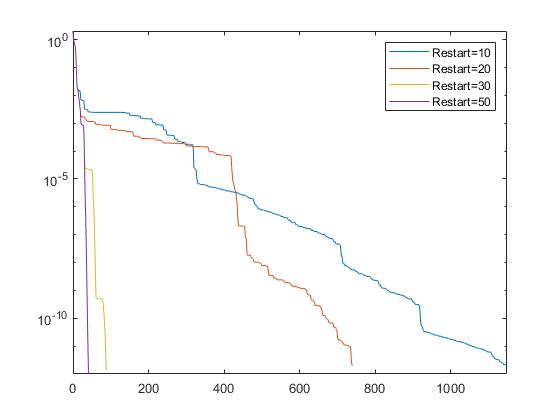
\includegraphics[width=.6\linewidth]{ex7.jpg}
			\caption{semilogy plot ex7}
			\label{fig:ex7}
		\end{figure}
	
		
		\section*{Question 8}
		
		\begin{table}[H]
			\centering
			\begin{tabular}{c|c|c|c|c|c|c}
				\textbf{Tolerance} & \textbf{Iterations} & \textbf{Tprec}  & \textbf{Tsol}  & \textbf{Ttotal} & \textbf{Final Residual} & \textbf{rho} \\ \hline
				$2 \times 10^{-2}$ & $1983$	& $ 39.59 s $ 	& $ 77.65 s $ & $ 117.24 s $ 	& $ 9.9053 \times 10^{-13} $ & $ 0.4537 $\\ \hline
				$1 \times 10^{-2}$ & $691$	& $ 36.46 s $ 	& $ 26.63 s $ & $ 63.09 s $ 	& $ 9.7254 \times 10^{-13} $ & $ 0.5807 $\\ \hline
				$3 \times 10^{-3}$ & $247$	& $ 40.67 s $ 	& $ 11.04 s $ & $ 51.71 s $ 	& $ 9.1709 \times 10^{-13} $ & $ 0.9401 $\\ \hline
				$1 \times 10^{-3}$ & $102$	& $ 37.61 s $ 	& $ 5.63 s $ & $ 43.24 s $ 		& $ 8.7501 \times 10^{-13} $ & $ 1.4544 $\\ \hline
				$1 \times 10^{-4}$ & $34$	& $ 42.44 s $ 	& $ 2.93 s $ & $ 45.37 s $ 		& $ 4.5169 \times 10^{-13} $ & $ 3.5140 $\\ \hline
				$1 \times 10^{-5}$ & $16$	& $ 76.50 s $ 	& $ 2.49 s $ & $ 78.99 s $ 		& $ 4.9947 \times 10^{-13} $ & $ 9.0720 $\\ \hline
			\end{tabular}
			\caption{Iterations for each value of nx, no preconditioning}
			\label{table:ex8}
		\end{table}
	
		
		
		\begin{figure}[H]
			\centering
			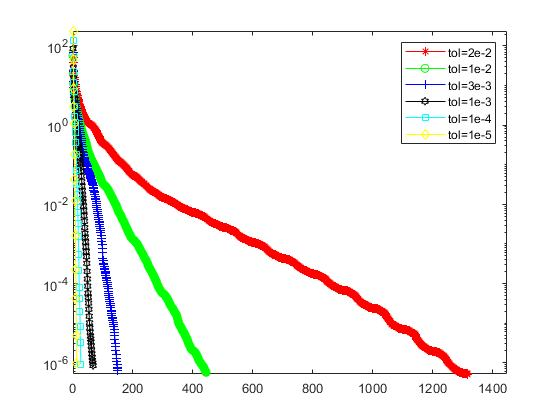
\includegraphics[width=.6\linewidth]{ex8.jpg}
			\caption{semilogy plot ex8}
			\label{fig:ex8}
		\end{figure}
	
	
	
\end{document}



